\section{Results}
\label{sec:results}

Unless stated otherwise, values in Sections~\ref{sec:res-internal}--\ref{sec:res-seeds} are from the selected model (version \RModelVersion, build \RDatasetBuild, checkpoint \texttt{\RCheckpointShort\ldots}, seed \RSeed), a single training run. Differences of a few percentage points between classes, sources or runs are within the range that seed variation could produce (Section~\ref{sec:res-seeds}) and should not be read as established. Run~2 was selected over run~1 by the rule of Section~\ref{sec:selection}: on the \RCmpN{} common selection images its macro-F1 was \RCmpRunTwoMacroFOne\% against \RCmpRunOneMacroFOne\% (accuracy \RCmpRunTwoAcc\% against \RCmpRunOneAcc\%, macro ROC-AUC \RCmpRunTwoMacroAUC{} against \RCmpRunOneMacroAUC). This comparison favours run~2 by construction. On the \RCmpRunOneSharedN{} common images from the four sources both runs trained on, accuracy was almost equal (\RCmpRunOneSharedAcc\% and \RCmpRunTwoSharedAcc\%) and the macro-F1 gap was much smaller (\RCmpRunOneSharedMacroFOne\% and \RCmpRunTwoSharedMacroFOne\%), so much of the advantage lies on TBX11K and COVID-19 Radiography images that are in-distribution for run~2 only. Of the paired predictions that differed in correctness, \RCmpMcNemarB{} were right for run~1 only and \RCmpMcNemarC{} for run~2 only. The full comparison is in Table~S4 of the supplement; with one seed per run it is no evidence that one recipe is better in general.

\subsection{Internal performance}
\label{sec:res-internal}
The run completed its full schedule of \REpochsTrained{} epochs; the selected checkpoint (epoch \RSelectedEpoch, the last) reached validation accuracy \RValAcc\%, macro-F1 \RValMacroFOne\% and macro ROC-AUC \RValMacroAUC. The validation curve was still rising slightly, and whether longer training would change the results was not tested. On the internal test split ($N=\RNTest$, evaluated once), accuracy was \RTestAcc\% (Wilson 95\% interval \RTestAccLo--\RTestAccHi\%), macro-F1 \RTestMacroFOne\%, macro ROC-AUC \RTestMacroAUC{} and ECE \RTestECE. The strongest classes by F1 were COVID-19 (\RFOneCovid\%), Tuberculosis (\RFOneTB\%) and Pneumonia (\RFOnePneumonia\%); the weakest were Pulmonary Nodule/Mass (\RFOneNodule\%) and Normal (\RFOneNormal\%). Nodule/Mass and Pleural Effusion come only from NIH, whose labels are mined from reports, so label noise and the subtlety of small nodules are both plausible contributors, which this study cannot separate. Per-class results are in Table~S3. A low ECE on the internal test split does not imply calibrated scores at another hospital.

Table~\ref{tab:persource} gives test accuracy within each source. Accuracy ranged from \RSrcAccCohen\% (COVID-19 image data collection) to \RSrcAccCovidRad\% (COVID-19 Radiography Database, which contributes one class). NIH, which supplies four classes including the two NIH-only classes, reached \RSrcAccNIH\%, whereas Kermany and TBX11K reached \RSrcAccKermany\% and \RSrcAccTBXk\%. Normal radiographs from NIH were called Normal far less often than Normal radiographs from Kermany, Shenzhen or TBX11K. The overall accuracy is a weighted mixture of these values and would change with the source mix. The pattern is consistent with source-specific appearance contributing to decisions, but per-source accuracy cannot separate a source effect from a difference in case mix.

\begin{table}[t]
\centering
\caption{Accuracy of the selected model within each source of the internal test split. ``Classes'' lists the classes the source contributes to the test split.}
\label{tab:persource}
\small
\begin{tabular}{@{}llrr@{}}
\toprule
Source & Classes & $N$ & Accuracy (\%) \\
\midrule
NIH ChestX-ray14 & Normal, Effusion, Pneumonia, Nodule/Mass & \RSrcNNIH & \RSrcAccNIH \\
Kermany (paediatric) & Normal, Pneumonia & \RSrcNKermany & \RSrcAccKermany \\
COVID-19 Radiography Database & COVID-19 & \RSrcNCovidRad & \RSrcAccCovidRad \\
TBX11K & Normal, Tuberculosis & \RSrcNTBXk & \RSrcAccTBXk \\
Shenzhen & Normal, Tuberculosis & \RSrcNShenzhen & \RSrcAccShenzhen \\
COVID-19 image data collection & COVID-19, Normal, Pneumonia, TB & \RSrcNCohen & \RSrcAccCohen \\
\bottomrule
\end{tabular}
\end{table}

\subsection{External cohort}
\label{sec:res-ext}
On Montgomery ($N=\RNExternal$, scored once), \RExtSensK{} of \RExtSensN{} TB radiographs were predicted as some class other than Normal (sensitivity \RExtSens\%, Wilson 95\% interval \RExtSensLo--\RExtSensHi\%) and \RExtSpecK{} of \RExtSpecN{} normal radiographs were predicted Normal (specificity \RExtSpec\%, interval \RExtSpecLo--\RExtSpecHi\%). The ROC-AUC of $1-p_{\text{Normal}}$ was \RExtAUC. Only \RExtTBK{} of \RExtTBN{} TB radiographs (\RExtTB\%) were assigned Tuberculosis, against an internal Tuberculosis recall of \RRecallTB\%, and COVID-19 was assigned to \RExtCovidCalls{} of the \RNExternal{} scans although the cohort contains no COVID-19 case. Fig.~\ref{fig:external} shows that most scans, normal and TB alike, were assigned Pneumonia or Pulmonary Nodule/Mass. The high sensitivity therefore says little about TB detection, and the low specificity means that the model would flag most healthy patients from this hospital as abnormal. That the abnormality score ranks above chance while specificity is low suggests that the decision boundary learned on the development sources does not transfer.

Run~1, evaluated once on the same cohort, assigned COVID-19 to \RRunOneExtCovidCalls{} scans, called \RRunOneExtSpecK{} of \RExtSpecN{} normal scans Normal and named \RRunOneExtTBK{} of \RExtTBN{} TB scans Tuberculosis. With build~2, which changed several sources at once, the COVID-19 calls fell from \RRunOneExtCovidCalls{} to \RExtCovidCalls. This is consistent with, but does not prove, run~1 having associated the appearance of its single COVID-19 source with the class. The external errors moved to other abnormal classes, specificity was lower than run~1's, and Tuberculosis was still not recognised. These are single-seed observations on one small cohort.

\begin{figure}[t]
\centering
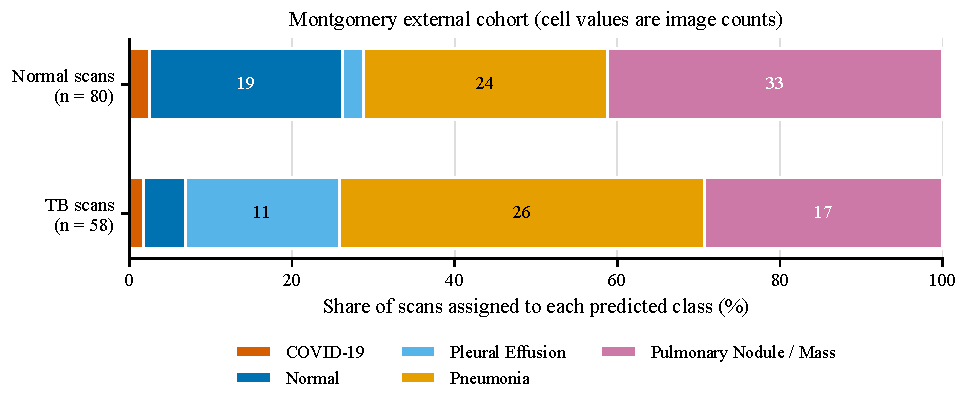
\includegraphics[width=\linewidth]{fig_external_breakdown.pdf}
\caption{Predicted class for the normal (left) and TB (right) radiographs of the external Montgomery cohort (selected model, scored once). The cohort contains no COVID-19, Pleural Effusion, Pneumonia or Nodule/Mass case.}
\label{fig:external}
\end{figure}

\subsection{Source-identifiability probe}
\label{sec:res-probe}
With ImageNet features the source was identified with balanced accuracy \RProbeImgBalAcc\% across \RProbeImgNSources{} sources (chance \RProbeImgChance\%; Table~\ref{tab:probe}), and it stayed identifiable within single classes: \RProbeImgWithinNormal\% among Normal images (chance \RProbeImgWithinNormalChance\%), \RProbeImgWithinTB\% among Tuberculosis, \RProbeImgWithinPneumonia\% among Pneumonia and \RProbeImgWithinCovid\% among COVID-19 images. Features of the trained backbone gave nearly identical values (\RProbeMdlBalAcc\% overall), as expected because fine-tuning changed only the last 17 weighted layers (verified by weight comparison). Source and class are confounded in this benchmark, and source information is linearly available in the features on which the classifier's head operates, so a source shortcut is possible. The probe does not show that the classifier uses it; we treat it as indirect evidence together with the per-source and external results.

\begin{table}[t]
\centering
\caption{Source-identifiability probe: balanced accuracy (\%) of a logistic regression predicting the source collection from frozen 1024-dimensional features on \RProbeNTest{} probe-test images (\RProbeNTrain{} probe-training images). ``Within'' rows use only images of that class. Chance is $1/S$ for $S$ sources.}
\label{tab:probe}
\small
\begin{tabular}{@{}lrrrr@{}}
\toprule
Images & Sources & Chance & ImageNet features & Trained backbone \\
\midrule
All classes & \RProbeImgNSources & \RProbeImgChance & \RProbeImgBalAcc & \RProbeMdlBalAcc \\
Within Normal & \RProbeImgWithinNormalNSources & \RProbeImgWithinNormalChance & \RProbeImgWithinNormal & \RProbeMdlWithinNormal \\
Within Tuberculosis & \RProbeImgWithinTBNSources & \RProbeImgWithinTBChance & \RProbeImgWithinTB & \RProbeMdlWithinTB \\
Within Pneumonia & \RProbeImgWithinPneumoniaNSources & \RProbeImgWithinPneumoniaChance & \RProbeImgWithinPneumonia & \RProbeMdlWithinPneumonia \\
Within COVID-19 & \RProbeImgWithinCovidNSources & \RProbeImgWithinCovidChance & \RProbeImgWithinCovid & \RProbeMdlWithinCovid \\
\bottomrule
\end{tabular}
\end{table}

\subsection{Seed variability and preprocessing ablation}
\label{sec:res-seeds}
Table~\ref{tab:seeds} reports the selected run and two further seeds (\RMSSeeds; \RMSNRuns{} runs on the same build, split and recipe). Internal results varied little: test accuracy had mean \RMSTestAccMean\% (SD \RMSTestAccSD, range \RMSTestAccMin--\RMSTestAccMax\%) and macro-F1 mean \RMSTestMacroFOneMean\% (SD \RMSTestMacroFOneSD, range \RMSTestMacroFOneMin--\RMSTestMacroFOneMax\%). The selected run is the highest of the three, within a spread of under one percentage point; a small favourable draw cannot be ruled out, and it was chosen before seeds \RMSRunTwoSeed{} and \RMSRunThreeSeed{} existed. External specificity varied more (mean \RMSExtSpecMean\%, range \RMSExtSpecMin--\RMSExtSpecMax\%), so differences of a few points in external specificity between runs of this recipe should not be interpreted. In every run, exact TB recall on Montgomery was \RMSExtTBMean\%, and specificity stayed low, so the external failure is consistent across seeds. The SD from three runs is a rough estimate and says nothing about other splits, data or architectures.

\begin{table}[t]
\centering
\caption{Seed variability of the selected configuration (build \RDatasetBuild). Test values in \%, except ROC-AUC; external specificity and exact TB recall in \%. Mean $\pm$ sample SD over three runs. The served model is run~2 regardless of these results.}
\label{tab:seeds}
\small
\begin{tabular}{@{}llrrrrr@{}}
\toprule
Run & Seed & Test acc. & Macro-F1 & Macro ROC-AUC & Ext. specificity & Ext. TB recall \\
\midrule
Run 2 (selected) & \RSeed & \RTestAcc & \RTestMacroFOne & \RTestMacroAUC & \RExtSpec & \RExtTB \\
Run 3 & \RMSRunTwoSeed & \RMSRunTwoTestAcc & \RMSRunTwoTestMacroFOne & \RMSRunTwoTestMacroAUC & \RMSRunTwoExtSpec & \RMSRunTwoExtTB \\
Run 4 & \RMSRunThreeSeed & \RMSRunThreeTestAcc & \RMSRunThreeTestMacroFOne & \RMSRunThreeTestMacroAUC & \RMSRunThreeExtSpec & \RMSRunThreeExtTB \\
\midrule
Mean $\pm$ SD & -- & \RMSTestAccMean{} $\pm$ \RMSTestAccSD & \RMSTestMacroFOneMean{} $\pm$ \RMSTestMacroFOneSD & \RMSTestMacroAUCMean{} $\pm$ \RMSTestMacroAUCSD & \RMSExtSpecMean{} $\pm$ \RMSExtSpecSD & \RMSExtTBMean{} $\pm$ \RMSExtTBSD \\
Min--max & -- & \RMSTestAccMin--\RMSTestAccMax & \RMSTestMacroFOneMin--\RMSTestMacroFOneMax & \RMSTestMacroAUCMin--\RMSTestMacroAUCMax & \RMSExtSpecMin--\RMSExtSpecMax & \RMSExtTBMin--\RMSExtTBMax \\
\bottomrule
\end{tabular}
\end{table}

In the preprocessing ablation (run~5, same seed, data and schedule, filters removed; Table~S6), test accuracy was \RAblTestAcc\% against \RMSRunOneTestAcc\% for the run with filters, macro-F1 \RAblTestMacroFOne\% against \RMSRunOneTestMacroFOne\% and macro ROC-AUC \RAblTestMacroAUC{} against \RMSRunOneTestMacroAUC. All three internal values lie below the whole seed range of runs 2--4, and the accuracy and macro-F1 differences are several times the seed SD, so in this single comparison the run with the filters scored higher internally by more than the seed-to-seed spread. External specificity was \RAblExtSpec\% against \RMSRunOneExtSpec\%, so removing the filters did not raise it. Run~5 named \RAblExtTB\% of the Montgomery TB scans Tuberculosis, a small number of scans, where no filtered run named any; this is an observation from one run. Run~5 also selected its last epoch (16 of 16, validation still rising), whereas runs 3 and 4 stopped early, so a difference in convergence speed cannot be excluded. With one ablation seed the difference cannot be separated from run-to-run variation outside the measured spread, and we make no claim about why the filters matter.

\subsection{C1: source and disease information by spatial-frequency band}
\label{sec:res-c1}
On the full cached image, ImageNet features gave source balanced accuracy \RSpecMainTestFullSrcBA\% (95\% interval \RSpecMainTestFullSrcBALo--\RSpecMainTestFullSrcBAHi\%; chance 16.7\%), within-source disease macro-F1 \RSpecMainTestFullFWs\%, six-class macro-F1 \RSpecMainTestFullFAll\% and within-Normal source accuracy \RSpecMainTestFullNormBA\% (test sample, $N=\RSpecMainTestN$; Table~\ref{tab:c1}, Fig.~\ref{fig:spectral}). The trained backbone and the no-filter cache gave source accuracy \RSpecServedTestFullSrcBA\% and \RSpecNofilterTestFullSrcBA\% and within-source macro-F1 \RSpecServedTestFullFWs\% and \RSpecNofilterTestFullFWs\% on the full image.

\textit{Source information is present in every band.} Band-pass source accuracy rose from \RSpecMainTestPassASrcBA\% in band A to \RSpecMainTestPassFSrcBA\% in band F, always above the 16.7\% chance level, with a dip at band B and a steep rise toward bands E and F. Within Normal images, source accuracy was \RSpecMainTestPassANormBA\% in band A and \RSpecMainTestPassFNormBA\% in band F, above the nominal 25\% in every band, so source information survives with disease held fixed. Disease information is also spread over the bands (within-source macro-F1 from \RSpecMainTestPassBFWs\% in band B to \RSpecMainTestPassFFWs\% in band F) and is highest in the high-frequency bands E and F, as is the source signal. Those bands may also be the ones most affected by resampling of different native grids and by the pre-filters.

\textit{No band is necessary.} Removing any single band left source accuracy nearly intact. The largest drop was \RSpecMainTestStopFDeltaS{} points for band F (interval \RSpecMainTestStopFDeltaSLo{} to \RSpecMainTestStopFDeltaSHi), the only band-stop whose interval excluded zero in that direction; removing band D shifted source accuracy the other way (\RSpecMainTestStopDDeltaS{} points, interval \RSpecMainTestStopDDeltaSLo{} to \RSpecMainTestStopDDeltaSHi). No band-stop reached the 5-point threshold fixed in advance, and all disease intervals included zero (the largest change was \RSpecMainTestStopEDeltaD{} points for band E). Source information is therefore redundant across bands in these features.

\textit{Sensitivity.} The profile of the trained backbone is close to the ImageNet profile (Fig.~\ref{fig:spectral}a). The no-filter cache shows the same shape, with a dip at band B and a rise toward E and F, but its levels differ: source accuracy is lower in the high bands (band E \RSpecNofilterTestPassESrcBA\% against \RSpecMainTestPassESrcBA\%, band F \RSpecNofilterTestPassFSrcBA\% against \RSpecMainTestPassFSrcBA\%, with non-overlapping intervals for band E) and slightly higher in bands A to C. This is consistent with the pre-filters and resampling contributing to the high-band source signal; it is a sensitivity result, not a test, and the per-band values of both checks are in Table~S7. The null result holds in all three: no band stands out as the carrier. Availability in frozen features does not show that the trained model uses the information.

\begin{table}[t]
\centering
\caption{C1 on the test sample (ImageNet features, primary; $N=\RSpecMainTestN$ images, \RSpecMainTestNWithinSources{} sources in the within-source score). Band-pass: source balanced accuracy with 95\% bootstrap interval over scored images, within-source disease macro-F1 and within-Normal source accuracy (\%). Band-stop: $dS$ and $dD$ are the full-image value minus the band-stop value in percentage points, with 95\% intervals. Chance for source accuracy is 16.7\%. One probe fit per variant; intervals cover test-sample variation only.}
\label{tab:c1}
\footnotesize
\setlength{\tabcolsep}{3pt}
\begin{tabular}{@{}lcrrcc@{}}
\toprule
 & \multicolumn{3}{c}{Band-pass} & \multicolumn{2}{c}{Band-stop} \\
\cmidrule(lr){2-4}\cmidrule(lr){5-6}
Band & Source acc. (95\% int.) & Within-source F1 & Within-Normal src. & $dS$ (95\% int.) & $dD$ (95\% int.) \\
\midrule
A & \RSpecMainTestPassASrcBA{} (\RSpecMainTestPassASrcBALo--\RSpecMainTestPassASrcBAHi) & \RSpecMainTestPassAFWs & \RSpecMainTestPassANormBA & \RSpecMainTestStopADeltaS{} (\RSpecMainTestStopADeltaSLo{} to \RSpecMainTestStopADeltaSHi) & \RSpecMainTestStopADeltaD{} (\RSpecMainTestStopADeltaDLo{} to \RSpecMainTestStopADeltaDHi) \\
B & \RSpecMainTestPassBSrcBA{} (\RSpecMainTestPassBSrcBALo--\RSpecMainTestPassBSrcBAHi) & \RSpecMainTestPassBFWs & \RSpecMainTestPassBNormBA & \RSpecMainTestStopBDeltaS{} (\RSpecMainTestStopBDeltaSLo{} to \RSpecMainTestStopBDeltaSHi) & \RSpecMainTestStopBDeltaD{} (\RSpecMainTestStopBDeltaDLo{} to \RSpecMainTestStopBDeltaDHi) \\
C & \RSpecMainTestPassCSrcBA{} (\RSpecMainTestPassCSrcBALo--\RSpecMainTestPassCSrcBAHi) & \RSpecMainTestPassCFWs & \RSpecMainTestPassCNormBA & \RSpecMainTestStopCDeltaS{} (\RSpecMainTestStopCDeltaSLo{} to \RSpecMainTestStopCDeltaSHi) & \RSpecMainTestStopCDeltaD{} (\RSpecMainTestStopCDeltaDLo{} to \RSpecMainTestStopCDeltaDHi) \\
D & \RSpecMainTestPassDSrcBA{} (\RSpecMainTestPassDSrcBALo--\RSpecMainTestPassDSrcBAHi) & \RSpecMainTestPassDFWs & \RSpecMainTestPassDNormBA & \RSpecMainTestStopDDeltaS{} (\RSpecMainTestStopDDeltaSLo{} to \RSpecMainTestStopDDeltaSHi) & \RSpecMainTestStopDDeltaD{} (\RSpecMainTestStopDDeltaDLo{} to \RSpecMainTestStopDDeltaDHi) \\
E & \RSpecMainTestPassESrcBA{} (\RSpecMainTestPassESrcBALo--\RSpecMainTestPassESrcBAHi) & \RSpecMainTestPassEFWs & \RSpecMainTestPassENormBA & \RSpecMainTestStopEDeltaS{} (\RSpecMainTestStopEDeltaSLo{} to \RSpecMainTestStopEDeltaSHi) & \RSpecMainTestStopEDeltaD{} (\RSpecMainTestStopEDeltaDLo{} to \RSpecMainTestStopEDeltaDHi) \\
F & \RSpecMainTestPassFSrcBA{} (\RSpecMainTestPassFSrcBALo--\RSpecMainTestPassFSrcBAHi) & \RSpecMainTestPassFFWs & \RSpecMainTestPassFNormBA & \RSpecMainTestStopFDeltaS{} (\RSpecMainTestStopFDeltaSLo{} to \RSpecMainTestStopFDeltaSHi) & \RSpecMainTestStopFDeltaD{} (\RSpecMainTestStopFDeltaDLo{} to \RSpecMainTestStopFDeltaDHi) \\
\midrule
Full image & \RSpecMainTestFullSrcBA{} (\RSpecMainTestFullSrcBALo--\RSpecMainTestFullSrcBAHi) & \RSpecMainTestFullFWs & \RSpecMainTestFullNormBA & -- & -- \\
\bottomrule
\end{tabular}
\end{table}

\begin{figure}[t]
\centering
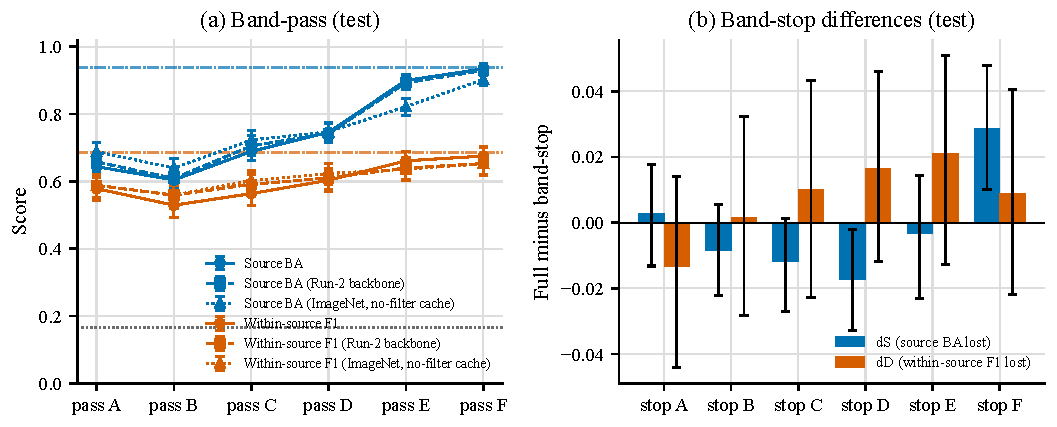
\includegraphics[width=\linewidth]{fig_spectral_map.pdf}
\caption{C1 on the test sample. (a) Band-pass variants A--F: source balanced accuracy (blue) and within-source disease macro-F1 (orange), both on the same score axis. Solid lines: ImageNet features (primary); dashed: run-2 backbone (secondary; it saw all six sources in training); dotted: ImageNet features of the no-filter cache (sensitivity check). The dotted grey horizontal line is the 16.7\% chance level for source accuracy; the dash-dot horizontal lines are the full-image levels of the primary extractor. (b) Band-stop differences, full image minus band-stop image, for source accuracy ($dS$) and within-source macro-F1 ($dD$). Error bars are 95\% bootstrap intervals over the scored images (one probe fit per variant; training variance is not included).}
\label{fig:spectral}
\end{figure}

\subsection{C3: linear erasure of source information}
\label{sec:res-c3}
Both extractors reached the cap of \RInlpImgKStar{} iterations ($k^\ast=\RInlpImgKStar$, stopped by the \RInlpImgStoppedBy), not the stopping threshold (Table~\ref{tab:inlp}, Fig.~\ref{fig:inlp}). With ImageNet features, the source balanced accuracy a fresh linear probe could reach fell from \RInlpImgTestSrcBAKZero\% at $k=0$ to \RInlpImgTestSrcBAKStar\% at $k^\ast$ on the test split ($N=\RInlpImgNTest$): a large reduction, but not to chance, so the source information was not removed by this linear route within the cap. Disease scores fell as well. The within-source macro-F1 changed by \RInlpImgTestChangeFWsKStar{} points (95\% interval \RInlpImgTestChangeFWsKStarLo{} to \RInlpImgTestChangeFWsKStarHi), the six-class macro-F1 by \RInlpImgTestChangeFAllKStar{} points (\RInlpImgTestChangeFAllKStarLo{} to \RInlpImgTestChangeFAllKStarHi), accuracy from \RInlpImgTestAccKZero\% to \RInlpImgTestAccKStar\% and macro ROC-AUC from \RInlpImgTestAUCKZero{} to \RInlpImgTestAUCKStar. Both intervals exclude zero, which is consistent with source and disease information being entangled in these features. The six-class drop exceeds the within-source drop, which is consistent with part of the six-class score being bought with source cues.

Removing all linearly decodable source information in a single step with LEACE (source accuracy at chance in the fit) lowered the six-class macro-F1 by \RInlpImgTestChangeFAllLeace{} points (compare the INLP loss at 20 iterations in the previous paragraph), and the within-source score by \RInlpImgTestChangeFWsLeace{} points. The trained backbone behaved similarly: source accuracy fell from \RInlpMdlTestSrcBAKZero\% to \RInlpMdlTestSrcBAKStar\% and the within-source macro-F1 changed by \RInlpMdlTestChangeFWsKStar{} points (\RInlpMdlTestChangeFWsKStarLo{} to \RInlpMdlTestChangeFWsKStarHi); these numbers come from a backbone that saw all sources and are not held-out results.

On Montgomery (Normal and Tuberculosis only, scored once; not untouched), ImageNet-feature heads had sensitivity \RInlpImgExtSensKZero\% (\RInlpImgExtSensKZeroK/\RInlpImgExtSensKZeroN) and specificity \RInlpImgExtSpecKZero\% (\RInlpImgExtSpecKZeroK/\RInlpImgExtSpecKZeroN) at $k=0$, and sensitivity \RInlpImgExtSensKStar\% and specificity \RInlpImgExtSpecKStar\% (Wilson interval \RInlpImgExtSpecKStarLo--\RInlpImgExtSpecKStarHi\%) at $k^\ast$. The specificity intervals overlap, the scans are the same at both settings so the intervals are not independent, and the cohort has 138 images; no conclusion about a change in specificity is drawn.

\begin{table}[t]
\centering
\caption{C3 on the full test split (ImageNet features, primary; $N=\RInlpImgNTest$). A fresh linear probe measures the source accuracy after projection; the disease head is retrained on the projected features. Percentages except ROC-AUC. LEACE: closed form, source accuracy at chance in the fit.}
\label{tab:inlp}
\small
\begin{tabular}{@{}lrrrrr@{}}
\toprule
Setting & Source acc. & Within-source F1 & Six-class macro-F1 & Accuracy & Macro ROC-AUC \\
\midrule
$k=0$ (no erasure) & \RInlpImgTestSrcBAKZero & \RInlpImgTestFWsKZero & \RInlpImgTestFAllKZero & \RInlpImgTestAccKZero & \RInlpImgTestAUCKZero \\
INLP, $k^\ast=\RInlpImgKStar$ & \RInlpImgTestSrcBAKStar & \RInlpImgTestFWsKStar & \RInlpImgTestFAllKStar & \RInlpImgTestAccKStar & \RInlpImgTestAUCKStar \\
LEACE & \RInlpImgLeaceTestSrcBA & \RInlpImgLeaceTestFWs & \RInlpImgLeaceTestFAll & \RInlpImgLeaceTestAcc & \RInlpImgLeaceTestAUC \\
\bottomrule
\end{tabular}
\end{table}

\begin{figure}[t]
\centering
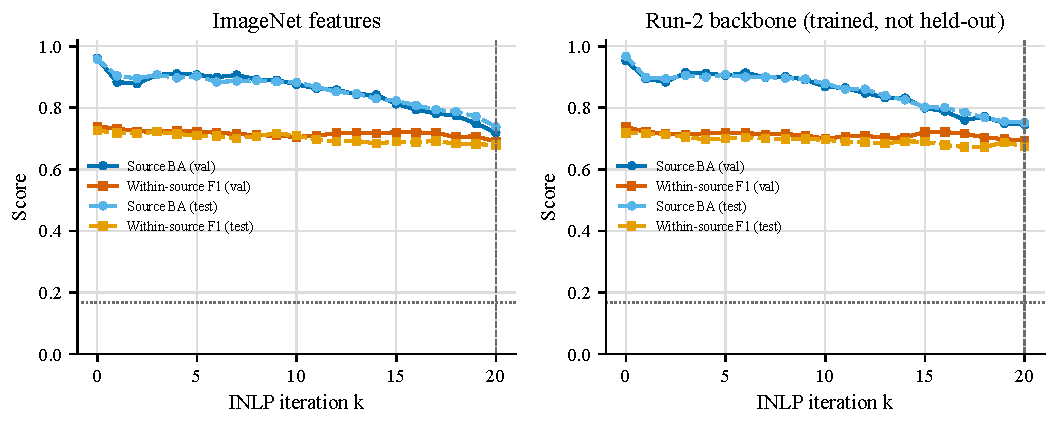
\includegraphics[width=\linewidth]{fig_inlp.pdf}
\caption{C3: source balanced accuracy of a fresh linear probe (blue) and within-source disease macro-F1 of the retrained head (orange) against INLP iteration $k$, on validation (solid) and test (dashed). Left: ImageNet features (primary). Right: run-2 backbone (secondary; trained on all six sources, so not held-out). The values at $k=0$ are the full-image levels without erasure. The dotted grey line is the 16.7\% chance level for source accuracy; the vertical dashed line marks the iteration cap of 20. Intervals are not drawn here; bootstrap 95\% intervals over test images for the changes at $k^\ast$ are given in the text.}
\label{fig:inlp}
\end{figure}

\subsection{C4: linear-head leave-one-source-out}
\label{sec:res-c4}
For \RLosoImgNIncluded{} sources, Table~\ref{tab:loso} and Fig.~\ref{fig:loso} give the macro-F1 of a linear head trained on the other five sources, on the evaluated classes of the held-out source, with the in-distribution reference and the gap (reference minus held-out). On four of the five sources the held-out score was far below the reference: the gap was \RLosoImgCohenGap{} points for the COVID-19 image data collection, \RLosoImgKermanyGap{} for Kermany, \RLosoImgShenzhenGap{} for Shenzhen and \RLosoImgTBXkGap{} for TBX11K, the largest. The trained-backbone matrix is similar (macro-F1 \RLosoMdlCohenMacroFOne\%, \RLosoMdlKermanyMacroFOne\%, \RLosoMdlShenzhenMacroFOne\% and \RLosoMdlTBXkMacroFOne\% for the same four sources) but is not a held-out test.

The NIH gap is negative (\RLosoImgNIHGap{} points, interval \RLosoImgNIHGapLo{} to \RLosoImgNIHGapHi; trained backbone \RLosoMdlNIHGap, interval \RLosoMdlNIHGapLo{} to \RLosoMdlNIHGapHi), but this is a metric artefact and should not be read as better generalisation. NIH has only two testable classes, and the six-class reference head also predicts the NIH-only classes Effusion and Nodule/Mass, which count as errors for the two evaluated classes; the reference is therefore low (\RLosoImgNIHRefMacroFOne\% with ImageNet features). Likewise, balanced accuracy below 50\% for a two-class source (TBX11K \RLosoImgTBXkBalAcc\%, COVID-19 image data collection \RLosoImgCohenBalAcc\%) reflects predictions of non-evaluated classes counted as errors, not a head worse than chance on a binary question. A chance-referenced reading comes from the binary abnormal-versus-normal view, in which the ROC-AUC of $1-P(\text{Normal})$ was \RLosoImgKermanyBinAUC{} for Kermany, \RLosoImgNIHBinAUC{} for NIH, \RLosoImgShenzhenBinAUC{} for Shenzhen and \RLosoImgTBXkBinAUC{} for TBX11K; the two TB sources, Shenzhen and TBX11K, are the lowest. This is consistent with dependence on source-specific cues and with class--source confounding, but it does not identify which cues. The COVID-19 image data collection has only \RLosoImgCohenN{} test images in its evaluated classes and its result is very uncertain.

Scored once with the head trained on all six sources, Montgomery gave sensitivity \RLosoImgExtSens\% and specificity \RLosoImgExtSpec\% with ImageNet features, and \RLosoMdlExtSens\% and \RLosoMdlExtSpec\% with the trained backbone (not untouched; 138 images). Every held-out number carries the patient-identity caveat of Section~\ref{sec:split}: TBX11K and COVID-19 Radiography rows are grouped per image and Kermany identities are derived from file names, so patient separation within those sources is not proven, and the reference scores in particular may be optimistic for them.

\begin{table}[t]
\centering
\caption{C4: macro-F1 (\%) on the evaluated classes of the held-out source for a linear head trained on the other five sources (ImageNet features, primary), with 95\% bootstrap interval over held-out test images, the in-distribution reference (head trained on all six sources, same images), the gap (reference minus held-out, in points) and the binary abnormal-versus-normal ROC-AUC where defined. Predictions of non-evaluated classes count as errors. $N$ is the number of test images in the evaluated classes.}
\label{tab:loso}
\small
\begin{tabular}{@{}lrcrrr@{}}
\toprule
Held-out source & $N$ & Held-out macro-F1 (95\% int.) & Reference & Gap & Binary AUC \\
\midrule
COVID-19 image data collection & \RLosoImgCohenN & \RLosoImgCohenMacroFOne{} (\RLosoImgCohenMacroFOneLo--\RLosoImgCohenMacroFOneHi) & \RLosoImgCohenRefMacroFOne & \RLosoImgCohenGap & -- \\
Kermany & \RLosoImgKermanyN & \RLosoImgKermanyMacroFOne{} (\RLosoImgKermanyMacroFOneLo--\RLosoImgKermanyMacroFOneHi) & \RLosoImgKermanyRefMacroFOne & \RLosoImgKermanyGap & \RLosoImgKermanyBinAUC \\
NIH ChestX-ray14 & \RLosoImgNIHN & \RLosoImgNIHMacroFOne{} (\RLosoImgNIHMacroFOneLo--\RLosoImgNIHMacroFOneHi) & \RLosoImgNIHRefMacroFOne & \RLosoImgNIHGap & \RLosoImgNIHBinAUC \\
Shenzhen & \RLosoImgShenzhenN & \RLosoImgShenzhenMacroFOne{} (\RLosoImgShenzhenMacroFOneLo--\RLosoImgShenzhenMacroFOneHi) & \RLosoImgShenzhenRefMacroFOne & \RLosoImgShenzhenGap & \RLosoImgShenzhenBinAUC \\
TBX11K & \RLosoImgTBXkN & \RLosoImgTBXkMacroFOne{} (\RLosoImgTBXkMacroFOneLo--\RLosoImgTBXkMacroFOneHi) & \RLosoImgTBXkRefMacroFOne & \RLosoImgTBXkGap & \RLosoImgTBXkBinAUC \\
\bottomrule
\end{tabular}
\end{table}

\begin{figure}[t]
\centering
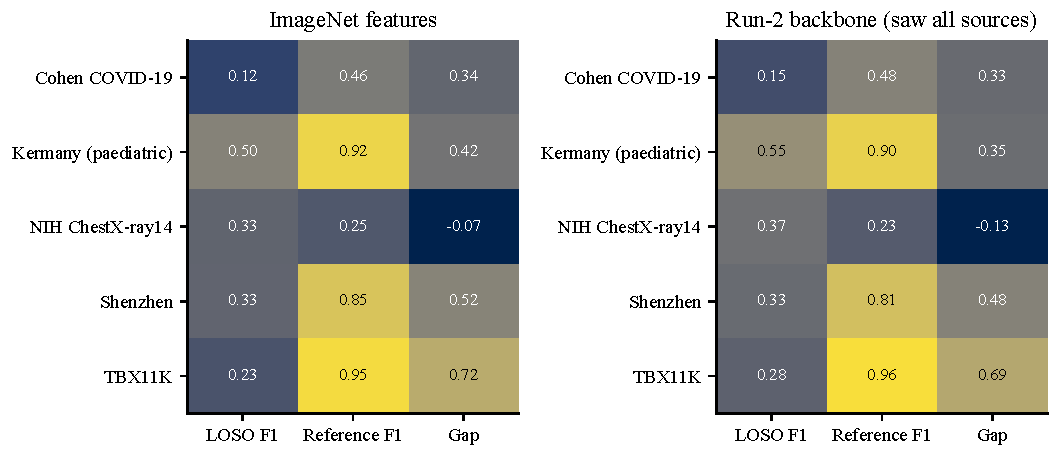
\includegraphics[width=\linewidth]{fig_loso_matrix.pdf}
\caption{C4: macro-F1 on the evaluated classes of the held-out source (``LOSO F1''; predictions of other classes count as errors), the in-distribution reference F1 and the gap (reference minus held-out), as fractions from 0 to 1 on one colour scale. Left: ImageNet features (primary). Right: run-2 backbone (secondary; it saw all six sources, so this is not a held-out or external test). Intervals are not drawn in the figure; 95\% bootstrap intervals over held-out test images are in Table~\ref{tab:loso}. The negative NIH gap is a metric artefact explained in the text. Patient-identity caveat: separation is proven only for rows with known identity.}
\label{fig:loso}
\end{figure}

\subsection{C2: decision not to retrain}
\label{sec:res-c2}
The go/no-go rule fixed in advance returned \RBsDecision. Criterion~1 \RBsConditionOne{} (\RBsNBandsSatisfying{} bands satisfied it; the band with the largest source drop was band \RBsBand), so the matched-energy random control was not run (criterion~2 \RBsConditionTwo), criterion~3 \RBsConditionThree{} and criterion~4 (the student's approval of compute) was moot. In the selection step for band \RBsBand{} the validation source-accuracy drop was \RSpecMainValStopFDeltaS{} points, below the 5-point threshold, and the upper bound of the disease change (\RSpecMainValStopFDeltaDHi{} points) also exceeded the 3-point limit. In the exploratory C2-lite step (ImageNet features, band \RBsBand{} removed, \RBsLiteValNTrain{} training images), the validation source-accuracy drop was \RBsLiteValDeltaS{} points (95\% interval \RBsLiteValDeltaSLo{} to \RBsLiteValDeltaSHi) and the disease change \RBsLiteValDeltaD{} points (\RBsLiteValDeltaDLo{} to \RBsLiteValDeltaDHi); on the test table, scored once and labelled exploratory, the values were \RBsLiteTestDeltaS{} points (\RBsLiteTestDeltaSLo{} to \RBsLiteTestDeltaSHi) and \RBsLiteTestDeltaD{} points (\RBsLiteTestDeltaDLo{} to \RBsLiteTestDeltaDHi). Removing the best single band thus lowered the source accuracy of a linear head by a few points, and the disease change was not distinguishable from zero. We report this as a negative result of the band-stop idea within this protocol and frozen features. No band-stop network was trained, so there is no C2 number and no statement about suppression in a trained network; C2 is future work.
